% Required report preamble:
% \usepackage{tikz}
% No additional TikZ libraries are required.

\chapter{Spritesheet Animation}
\label{chap:spritesheet-animation}

A spritesheet stores several animation frames in one PNG image. RatMan displays a selected rectangular region and changes it over time. The animation system belongs to \texttt{RatMan.App}; movement and game rules remain in the WPF-independent \texttt{RatMan.Game} library.

\section{Architecture}

Figure~\ref{fig:spritesheet-architecture} shows the main responsibilities. Sheet factories define the images and clips for RatMan, cats, and cheese. A \texttt{SpriteSheetDefinition} contains an image URI and named clips. Each \texttt{SpriteAnimationClip} contains an ordered list of frames and a looping flag; each \texttt{SpriteFrameDefinition} specifies a source rectangle and duration.

\begin{figure}[htbp]
    \centering
    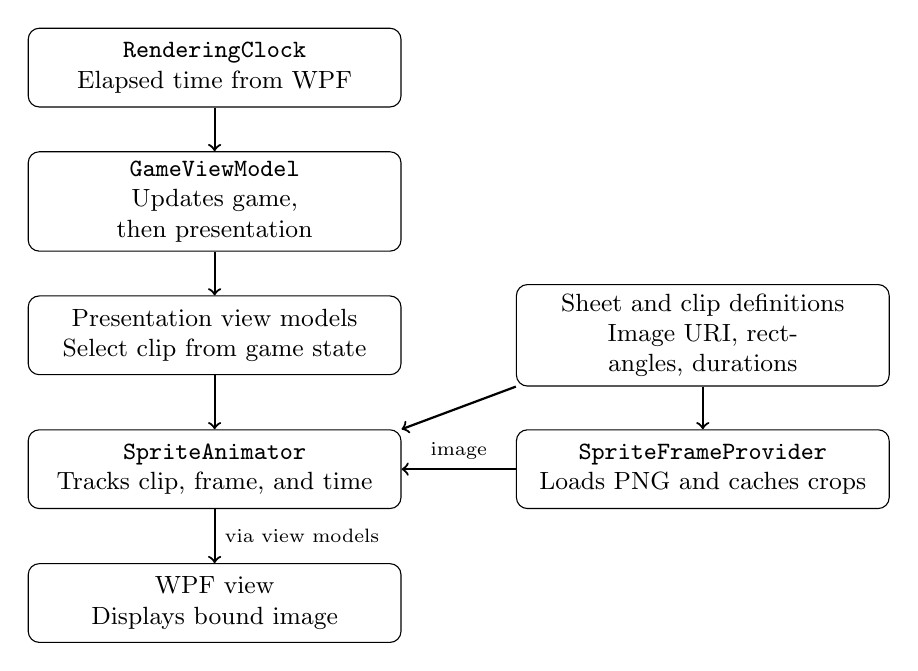
\begin{tikzpicture}[
        box/.style={draw, rounded corners, align=center, text width=4.5cm,
                    minimum height=1cm, font=\small},
        flow/.style={->, thick}
    ]
        % Explicit coordinates avoid a dependency on the positioning library.
        \node[box] (clock) at (0,0) {\texttt{RenderingClock}\\Elapsed time from WPF};
        \node[box] (game) at (0,-1.7) {\texttt{GameViewModel}\\Updates game, then presentation};
        \node[box] (presentation) at (0,-3.4) {Presentation view models\\Select clip from game state};
        \node[box] (animator) at (0,-5.1) {\texttt{SpriteAnimator}\\Tracks clip, frame, and time};
        \node[box] (definition) at (6.2,-3.4) {Sheet and clip definitions\\Image URI, rectangles, durations};
        \node[box] (provider) at (6.2,-5.1) {\texttt{SpriteFrameProvider}\\Loads PNG and caches crops};
        \node[box] (view) at (0,-6.8) {WPF view\\Displays bound image};

        \draw[flow] (clock) -- (game);
        \draw[flow] (game) -- (presentation);
        \draw[flow] (presentation) -- (animator);
        \draw[flow] (definition.south west) -- (animator.north east);
        \draw[flow] (definition) -- (provider);
        \draw[flow] (provider) -- node[above, font=\scriptsize] {image} (animator);
        \draw[flow] (animator) -- node[right, font=\scriptsize] {via view models} (view);
    \end{tikzpicture}
    \caption{Animation update and data flow. Arrows show information flow.}
    \label{fig:spritesheet-architecture}
\end{figure}

\section{Playback and Rendering}

\texttt{RenderingClock} uses WPF's rendering event and a stopwatch to supply elapsed time, capped at 100\,ms per update to limit jumps after a delay. After the game updates, the presentation view models select a clip using the actor's state and direction, for example \texttt{walking-left}. Position comes from the game model independently of the displayed sprite.

\texttt{SpriteAnimator.Advance} accumulates elapsed time and moves through as many frames as their durations require, retaining leftover time. Looping clips repeat; a non-looping clip holds its last frame and raises \texttt{Completed} once. Selecting an already active clip normally preserves playback. RatMan's blocked animation is instead restarted and advanced to the time derived from the game's remaining blocked duration.

\texttt{SpriteFrameProvider} loads the PNG once per provider, validates crop bounds, and caches each distinct rectangle as a frozen WPF image. Sheet factories share these resources while actors keep separate playback state. Optional padding gives irregular cat frames a common canvas size. Property-change notifications update the images bound in XAML.

This separation allows new clips to reuse the same playback code. The animator depends on \texttt{ISpriteFrameProvider}, so timing tests can substitute a fake provider without loading PNG files. Existing tests cover multi-frame advancement, looping, and completion of non-looping clips.
